\documentclass[aspectratio=169,10pt]{beamer}
\usepackage[english]{babel}
\usepackage[utf8]{inputenc}
\usepackage[T5,T1]{fontenc}
\usepackage[scaled=0.94]{helvet}
\renewcommand{\familydefault}{\sfdefault}
\usepackage{beamerthemeUET}
\usepackage{amsmath,amssymb,booktabs,tabularx,colortbl}
\usetikzlibrary{calc,arrows.meta}
\setbeamersize{text margin left=0.8cm,text margin right=0.8cm}
\setbeamerfont{normal text}{size=\normalsize}
\hypersetup{pdftitle={LIGHT WAVE DEHAZE},pdfauthor={Lương Duy Quân, Lê Minh Sơn, Nguyễn Khánh Việt},pdfsubject={Problem statement, existing approaches, and method objectives}}
\title[LIGHT WAVE DEHAZE]{LIGHT WAVE DEHAZE}
\subtitle{}
\author[Team Members]{\texorpdfstring{{\fontencoding{T5}\selectfont Lương Duy Quân\qquad Lê Minh Sơn\qquad Nguyễn Khánh Việt}}{Lương Duy Quân, Lê Minh Sơn, Nguyễn Khánh Việt}}
\date{}
\setunivname{}
% Keep the UET composition with the confirmed team members.
\newcommand{\key}[1]{\textbf{\color{uetblue}#1}}
\begin{document}

% 1. Cover with the team members supplied by the user.
\begin{frame}[plain]
  \titlepage
\end{frame}

\section{Problem Statement}
% 2. Problem and motivation.
\begin{frame}{Problem Statement}
  \vspace{-0.06cm}
  \[
    I(x)=J(x)t(x)+A\bigl[1-t(x)\bigr]
  \]
  \vspace{-0.13cm}
  \begin{columns}[T,onlytextwidth]
    \begin{column}{0.48\textwidth}
      \centering
      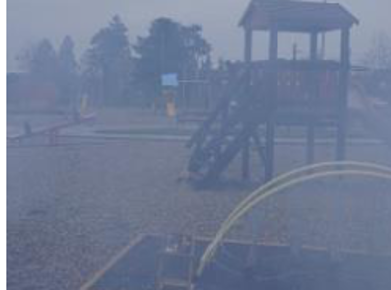
\includegraphics[height=2.65cm]{assets/hazy.png}\\[3pt]
      {\small\key{Hazy image $I$}}
    \end{column}
    \begin{column}{0.48\textwidth}
      \centering
      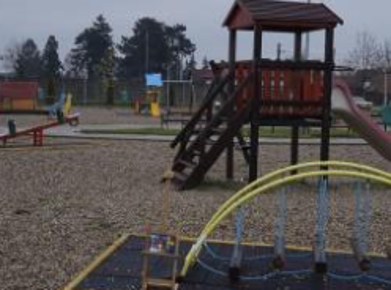
\includegraphics[height=2.65cm]{assets/clean.png}\\[3pt]
      {\small\key{Clean image $J$}}
    \end{column}
  \end{columns}
  \vspace{0.22cm}
  \begin{itemize}
    \item Recover a clean image from a single hazy observation.
  \end{itemize}
  % Reference: Midterm slides, p. 2.
\end{frame}

% 3. Both illustrations are extracted directly from source page 3.
\begin{frame}{Why Dehazing Is Needed}
  \begin{columns}[T,onlytextwidth]
    \begin{column}{0.39\textwidth}
      {\small\key{Haze obscures distant objects}}\par
      \vspace{0.20cm}
      \centering
      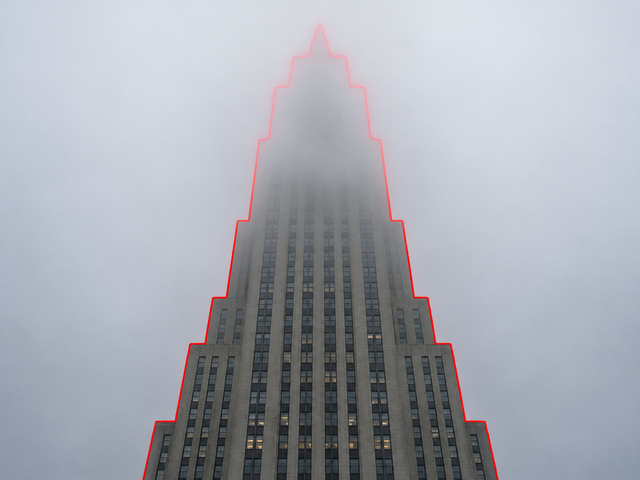
\includegraphics[width=\linewidth,height=3.65cm,keepaspectratio]{assets/haze-obscures-objects.png}
    \end{column}
    \begin{column}{0.58\textwidth}
      {\small\key{Preprocessing for detection and tracking}}\par
      \vspace{0.20cm}
      \centering
      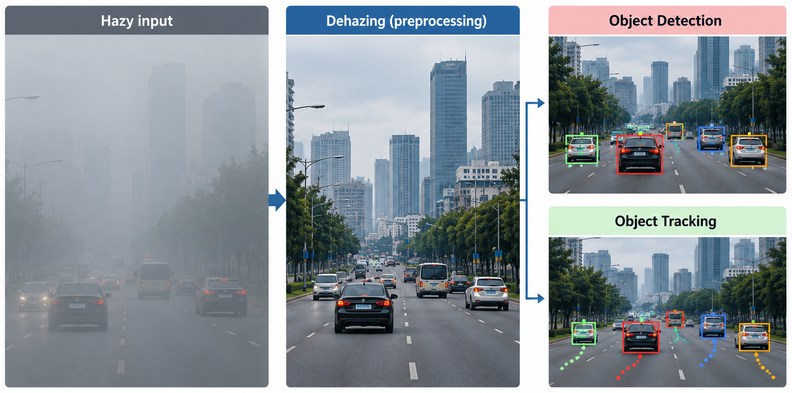
\includegraphics[width=\linewidth,height=3.65cm,keepaspectratio]{assets/dehazing-detection-tracking.png}
    \end{column}
  \end{columns}
  \vspace{0.23cm}
  % Reference: Images and application examples from Midterm slides, p. 3.
\end{frame}

\section{Existing Approaches}
% 4. Keep the four method families named on source page 4.
\begin{frame}{Existing Dehazing Approaches}
  \vspace{0.14cm}
  {\small\color{uetdark}
  \renewcommand{\arraystretch}{1.35}
  \begin{tabular}{@{}>{\raggedright\arraybackslash}p{2.7cm} >{\raggedright\arraybackslash}p{5.35cm} >{\raggedright\arraybackslash}p{5.25cm}@{}}
    \toprule
    \rowcolor{uetaccentbg}
    \key{Approach} & \key{Core idea} & \key{Key consideration}\\
    \midrule
    \textbf{Physical Prior} & Restore images using assumptions about haze and the scene & Depend on how well the assumptions match the scene\\
    \textbf{CNN} & Learn features through convolution & Ability to capture wider context\\
    \textbf{Transformer} & Model relationships across image regions & Computational and memory costs\\
    \textbf{Diffusion} & Restore images through denoising & Latency with multiple inference steps\\
    \bottomrule
  \end{tabular}}\par
  \vspace{0.25cm}
  {\small\color{uetgray}Trade-offs depend on the architecture and its optimization.}
  % Reference: Method families from Midterm slides, p. 4. CNN: convolutional neural network.
\end{frame}

\section{Problem Statement}
% 5. Inserted after Existing Dehazing Approaches, following source page 5.
\begin{frame}{Combining Strengths}
  \begin{columns}[c,onlytextwidth]
    \begin{column}{0.74\textwidth}
      \centering
      {\fontsize{16pt}{24pt}\selectfont\bfseries\color{uetdark}
      How can we use the strengths\\
      of each method at different stages\\
      of image processing?\par}
    \end{column}
    \begin{column}{0.22\textwidth}
      \centering
      
\includegraphics[height=3.5cm,keepaspectratio]{assets/combining-strengths-question.png}
    \end{column}
  \end{columns}
  % Reference: Question from Midterm slides, p. 5.
  % Replacement icon: Twemoji 14.0.2, 2753.svg, Twitter, Inc. and contributors, CC-BY 4.0.
  % https://github.com/twitter/twemoji/blob/v14.0.2/assets/svg/2753.svg
\end{frame}

\section{Motivation \& Key Insight}
% 6. Original DWT illustration, including its existing English labels.
\begin{frame}{Frequency-Domain Observation}
  \begin{columns}[c,onlytextwidth]
    \begin{column}{0.66\textwidth}
      \centering
      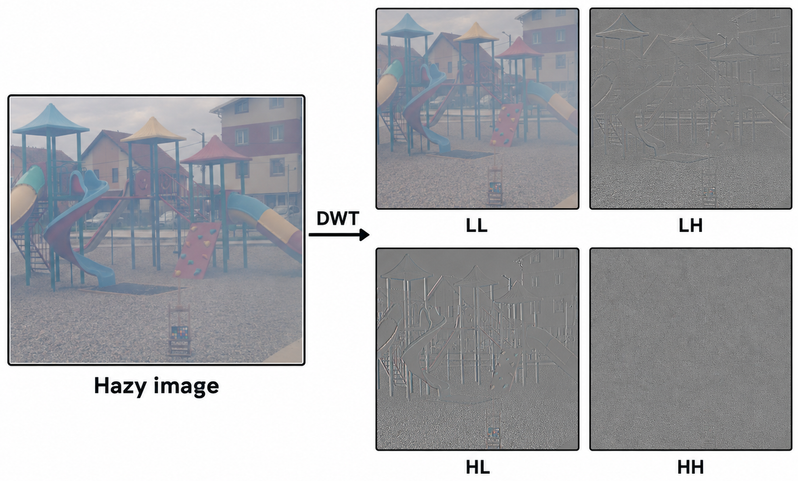
\includegraphics[width=\linewidth,height=4.9cm,keepaspectratio]{assets/dwt-frequency-observation.png}
    \end{column}
    \begin{column}{0.31\textwidth}
      {\small
      \key{Low-frequency component (LL)}\par
      Global appearance and scene structure.
      \vspace{0.32cm}\par
      \key{High-frequency components}\par
      Edges and local details in LH, HL, and HH.
      \vspace{0.32cm}\par
      \key{Key idea}\par
      Match each method's strengths to its restoration stage.}
    \end{column}
  \end{columns}
  % Reference: Original DWT illustration from Midterm slides, p. 6. Motivation and design from pp. 5 and 8.
\end{frame}

\section{Proposed Method}
% 7. Combined method overview and objectives, without repeated module descriptions.
\begin{frame}{Overall Design and Objectives}
  \centering
  % Schematic overview, not a layer-by-layer implementation.
% Method: supplied midterm deck, pp. 8, 10--11.
% Input/output photographs cropped from the supplied overview artwork.
\begin{tikzpicture}[
  x=1cm,y=1cm,
  font=\sffamily\fontsize{10}{13}\selectfont,
  module/.style={draw=uetblue,line width=0.8pt,fill=white,
    minimum width=3.90cm,minimum height=2.25cm,text width=3.60cm,
    align=center,inner sep=0.15cm,text=uetdark},
  flow/.style={-{Latex[length=2.2mm,width=1.5mm]},
    draw=uetdark,line width=0.85pt},
  stage/.style={font=\sffamily\fontsize{10}{12}\selectfont\bfseries,
    text=uetblue,align=center},
  image label/.style={font=\sffamily\fontsize{10}{13}\selectfont,
    text=uetdark,align=center}
]
  % Uniform module sizes and balanced connector gaps: 0.75 / 0.8 / 0.75 cm.
  \node[inner sep=0pt] (input) at (0.95,0)
    {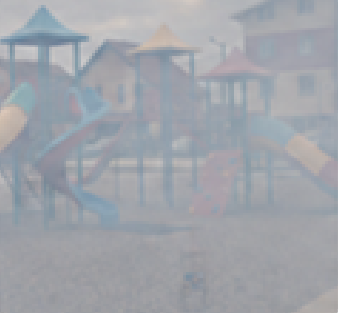
\includegraphics[width=1.90cm,height=1.76cm]{assets/overview-hazy-input.png}};
  \node[module] (lfrn) at (4.60,0)
    {\textbf{\large LFRN}\\[7pt]
     Low-frequency recovery\\[4pt]
     {\color{uetgray}Mamba on LL}};
  \node[module,draw=uetdarkgreen] (den) at (9.30,0)
    {\textbf{\large DEN}\\[7pt]
     Detail enhancement\\[4pt]
     {\color{uetgray}Spatial + frequency}};
  \node[inner sep=0pt] (output) at (12.95,0)
    {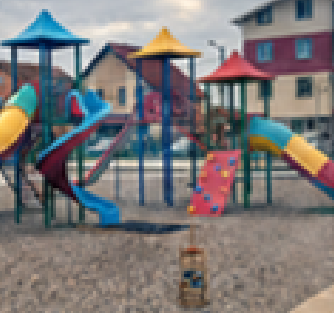
\includegraphics[width=1.90cm,height=1.76cm]{assets/overview-restored-output.png}};

  \draw[flow] ([xshift=3pt]input.east) -- ([xshift=-3pt]lfrn.west);
  \draw[flow] ([xshift=3pt]lfrn.east) --
    node[above=5pt,text=uetdark] {$\widetilde{I}$}
    ([xshift=-3pt]den.west);
  \draw[flow] ([xshift=3pt]den.east) -- ([xshift=-3pt]output.west);

  \node[stage,text width=3.90cm] at (4.60,1.75)
    {Stage 1\\[2pt]Global restoration};
  \node[stage,text=uetdarkgreen,text width=3.90cm] at (9.30,1.75)
    {Stage 2\\[2pt]Detail refinement};
  \node[image label,anchor=base] at (0.95,-1.22) {Hazy input};
  \node[image label,anchor=base] at (12.95,-1.22) {Restored image};
  \node[image label,anchor=base] at (0.95,-1.72) {$I_{\mathrm{h}}$};
  \node[image label,anchor=base] at (12.95,-1.72) {$\widehat{I}$};
\end{tikzpicture}

  \par\vspace{0.32cm}
  \begin{itemize}
    \setlength{\itemsep}{0.16cm}
    \item \key{Restoration:} remove global haze while preserving local details.
    \item \key{Efficiency:} balance restoration quality with inference cost.
  \end{itemize}
  \raggedright
  % Reference: Midterm slides, pp. 8, 10--11, and 14--15.
\end{frame}

\section{Evaluation}
% 8. Introduce each metric before presenting the proposed thresholds.
\begin{frame}{Evaluation Metrics}
  \par\vspace{0.14cm}
  {\small\color{uetdark}
  \renewcommand{\arraystretch}{1.55}
  \begin{tabular}{@{}>{\raggedright\arraybackslash}p{1.85cm} >{\raggedright\arraybackslash}p{6.50cm} >{\raggedright\arraybackslash}p{4.80cm}@{}}
    \toprule
    \rowcolor{uetaccentbg}
    \key{Metric} & \key{What it measures} & \key{How to interpret it}\\
    \midrule
    \textbf{PSNR (dB)} & Peak signal-to-noise ratio\newline Pixel accuracy against a clean reference. & Higher values indicate lower pixel error.\\
    \midrule
    \textbf{SSIM} & Structural similarity index\newline Compares structure, contrast, and luminance with a clean reference. & Values closer to 1 indicate greater similarity.\\
    \midrule
    \textbf{FPS} & Frames per second\newline Number of images processed per second. & Higher values indicate faster processing.\\
    \bottomrule
  \end{tabular}}\par
  \vspace{0.25cm}
  {\small\color{uetgray}Compare FPS using the same hardware, image resolution, and batch size.}
  % Metric definitions: scikit-image metrics documentation (PSNR and SSIM).
  % https://scikit-image.org/docs/stable/api/skimage.metrics.html
  % FPS is throughput; the measurement setup must be held constant.
\end{frame}

% 9. Keep proposal targets clearly separate from the source method.
\begin{frame}{Further Optimization Targets}
  {\small\key{Targets on the SOTS dataset}}
  \vspace{0.24cm}
  \begin{columns}[T,onlytextwidth]
    \begin{column}{0.30\textwidth}
      \statcard[uetblue]{$\geq 25\,\text{dB}$}{PSNR}
    \end{column}
    \begin{column}{0.30\textwidth}
      \statcard[uetgreen]{$\geq 0.95$}{SSIM}
    \end{column}
    \begin{column}{0.30\textwidth}
      \statcard[uetcyan]{$\geq 20$}{FPS}
    \end{column}
  \end{columns}
  \vspace{0.30cm}
  \begin{itemize}
    \setlength{\itemsep}{0.13cm}
    \item Optimize the frequency-domain and RGB restoration blocks.
    \item Assess latency, parameters, and FLOPs for future edge deployment.
  \end{itemize}
  \vspace{0.10cm}
  {\scriptsize\color{uetgray}Proposed targets, not reported results. Specify the hardware and image resolution for FPS.}
  % Reference: Preliminary research proposal, pp. 1--2.
\end{frame}

% 10. Closing slide.
\begin{frame}[c]
  \centering
  {\fontsize{28pt}{34pt}\selectfont\bfseries\color{uetblue}Thank You\par}
  \vspace{0.35cm}
  {\large\color{uetdarkgreen}Questions and Discussion\par}
\end{frame}
\end{document}
